\documentclass{standalone}

\usepackage{tikz}
\usepackage{amssymb}
\usetikzlibrary{calc, positioning, intersections}
\begin{document}
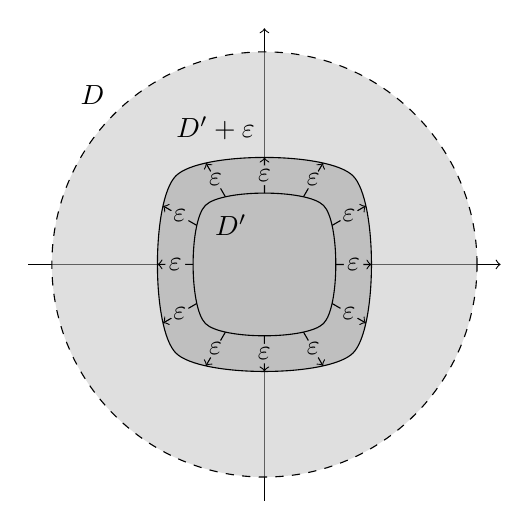
\begin{tikzpicture}[scale=1.5]
	\draw[->] (-2,0) to (2,0);
	\draw[->] (0,-2) to (0,2);
	\draw[dashed, fill=gray!50, fill opacity=0.5] (0,0) circle (1.8);
	\node[above left] at (135:1.8) {$ D $ };

	\def\area[scale=#1, name=#2]{
		\draw[fill=gray!50, name path=#2]
		plot[smooth cycle] coordinates {(-#1,-#1) (#1,-#1) (#1,#1) (-#1,#1)};
		\path[name path=circle] foreach \i in {0, 30, ..., 330} {(0,0) --({\i:#1+0.4})};
		\path[name intersections={of=#2 and circle, name=#2, total=\t}];
	}

	\def\outer{0.75}
	\def\inner{0.5}
	\area[scale=\outer, name=o];
	\area[scale=\inner, name=i];

	\foreach \p in {1,...,12}{
			\draw[->] (i-\p) to node[fill=gray!50, circle, inner sep=0.01cm] {$
					\varepsilon $} (o-\p);
		}

	\node[left] at (0,{\outer+0.4}) {$ D' + \varepsilon $};
	\node[below right] at (-\inner, \inner) {$ D' $};

\end{tikzpicture}
\end{document}
